%
% Manchester Raspberry Jam Workshop Booklet
%
% This template is designed to try and aide consistency between each booklet.
% Insert files and settings only as instructed by comments.
%

% Is this document PRINT or WEB format?
% use \printtrue or \printfalse
\newif\ifprint
\printtrue

% Page Formatting
\ifprint
	\documentclass[a4paper, twocolumn, twoside, 11pt]{article}
	\usepackage[margin=2cm]{geometry}
	\setlength{\columnsep}{1.25cm}
	\setlength{\parskip}{6pt}
\else
	\documentclass[a4paper, onecolumn, oneside, 11pt]{article}
	\usepackage[margin=3cm]{geometry}
	\setlength{\parskip}{9pt}
\fi



% FONT and text format
\usepackage[utf8x]{inputenc}	
\usepackage[UKenglish]{babel}
\ifprint
	\usepackage[usenames, dvipsnames]{color}				%Font Colour
	\usepackage[colorlinks=false]{hyperref}	%URLs
\else
	\usepackage[T1]{fontenc}
	\usepackage[sfdefault]{roboto}
	\usepackage[T1]{fontenc}
	\usepackage[usenames, dvipsnames]{color}				%Font Colour
	\usepackage[colorlinks=true,linkcolor=black,urlcolor=WildStrawberry]{hyperref}
\fi



% Table of Contents Format
\usepackage{tocloft}
\addtocontents{toc}{\cftpagenumbersoff{subsection}}
\setcounter{tocdepth}{2}
\setcounter{secnumdepth}{2}



% Section spacing
\ifprint
	\usepackage[compact]{titlesec}
\fi



% Listings and Asides
\usepackage{McrRaspJam/common/listings}
\usepackage{McrRaspJam/common/asides}



%Clear page for web version
\newcommand{\webclearpage}{
	\ifprint
	\else
		\clearpage
	\fi
}

% misc.
\usepackage{enumitem}									%List spacing changes
\usepackage[toc,page]{appendix}							%Appendix package
\usepackage{graphicx}									% TOC?
\usepackage{etoolbox}									%Boolean used for print/web switching
\usepackage{fancyvrb}									%Centered verbatim

% Enter the document title here
\newcommand{\workshopTitle}{Workshop 16: Ciphers}

% Enter the author of this workshop
\newcommand{\workshopAuthor}{Written by Jack Kelly}


\begin{document}
	% Title Format
\ifprint
	\title{Manchester Raspberry Jam \\ \workshopTitle}
	\author{}
\else
	\title{
		\begin{center}
			
\includegraphics[width=30mm]{McrRaspJam/common/logo-512}
		\end{center}
		\vspace{12pt}
		\workshopTitle
	}
	\author{
		Written by \workshopAuthor
	}
\fi

\date{\vspace{-16pt}}
\maketitle


% Online download location
\ifprint
	\begin{mdframed}[rightline=false, leftline=false]
		\scriptsize
		This booklet is available online at \mbox{\href{https://drive.google.com/open?id=0B_1SFjX_5JrmfnhpX0pPRXl6bmJNal8zdUxMeWZOdjJyZVdzU3V6UnBGdlVIMENtbFFkbVk}{bit.ly/McrRaspJam}}
		\normalsize
	\end{mdframed}
\fi
	
	%Place a SINGLE paragraph summary here
	Learn how classical ciphers worked to enable secretive communication, and learn how to write Python programs to encode, decode and crack them!
	
	%Difficulty
	\textit{Difficulty: Introductory workshop.}
	
	\ifprint
		\renewcommand{\baselinestretch}{0.75}\normalsize
		\tableofcontents
		\renewcommand{\baselinestretch}{1.0}\normalsize
	\else
		\tableofcontents
	\fi
	
	%
	% Input the main CONTENT below, sans title page or contents.
	% Recommend inputting per section, and adding page breaks here.
	%
	% \webclearpage command is provided, will break page for web format only.
	%
	
	\setcounter{section}{-1}
\section{Introduction}

	Last month in \href{http://mcrraspjam.org.uk/workshop-15-gpio-zero/}{workshop 15}, we \textit{encoded} a message in Morse code, a method that makes it simpler to transmit written language through rudimentary means, such as a spotlight, or a pulse in an electrical wire.
	
	We also often use the word \textit{code} to refer to an encrypted \textbf{cipher}. A different type of encoding, when we encode a message in a cipher, we attempt to make the message difficult---or ideally impossible--- for an outsider to read.
	
	Today, we'll have a go at encoding, decoding and cracking some famous ciphers of the classical era using Python programs, as well as taking a look at more modern ciphers and some of the cryptography tools available to us as users of Linux on the Raspberry Pi.
	
	
	%Difficulty
	This is an introductory workshop, all of the Python concepts will be covered from scratch.
		
	\subsection*{How to use these booklets}

	The aim of these booklets is to help you attempt these workshops at home, and to explain concepts in more detail than at the workshop. You don't need to follow these booklets during the workshop, but you can if you'd like 0to.
	
	%Code Listings
		When you need to make changes to your code, they'll be presented in \textit{listings} like the example below. Some lines may be repeated across multiple listings, so check the line numbers to make sure you're not copying something twice.

	\lstinputlisting[style=Python, lastline=2]{McrRaspJam/015_GPIOZero/0_introduction/led.py}
	
	
	
	Occasionally, a concept will be explained in greater detail in \textit{asides}, like the one below. You can read these as you wish, but they're not required to complete the workshop.
	
\begin{aside}[Resistors]
	Resistors are most commonly used to limit the amount of current flowing through part of an electrical circuit.
	
	For example we use resistors in series with LEDs, as otherwise they could draw so much power that they destroy themselves.
	
	Buttons have almost no internal resistance, so we use high value ($\sim 10  k\Omega$) resistors to prevent current flowing straight from the power supply to ground; if we didn't, the entire CPU could be short circuited, and the Pi would lose power!
\end{aside}
	
	\ifprint\else
		\subsection*{What you'll need}
		All of the software you for this workshop is pre-installed on recent versions of Raspbian.
	\fi
		
	\subsection*{Everything else}
	
		% Aknowledgements
		These booklets were created using \textrm{\LaTeX}, an advanced typesetting system used for several sorts of books, academic reports and letters.
			
		\ifprint\else If you'd like to have a look at using LaTeX, We recommend looking at \TeX studio, which is available on most platforms, and also in the Raspbian repository. \fi
		
		% License spiel
		To allow modification and redistribution of these booklets, they are distributed under the \hbox{CC BY-SA 4.0} License.
		Latex source documents are available at \url{http://github.com/McrRaspJam/booklet-workshops}
		
		If you get stuck, find errors or have feedback about these booklets, please email me at:
		\href{mailto:jam@jackjkelly.com}{\texttt{jam@jackjkelly.com}}

	\clearpage
	\section{Python Basics}

	In order to write programs to perform cryptography, we will need to be able to manipulate words and sentences, which in programming we call \textit{strings}.
	
	We'll start with some basic Python programs, which will teach us everything we need in order to pull words and sentences apart.
	
	\begin{figure}[h]
		\centering
		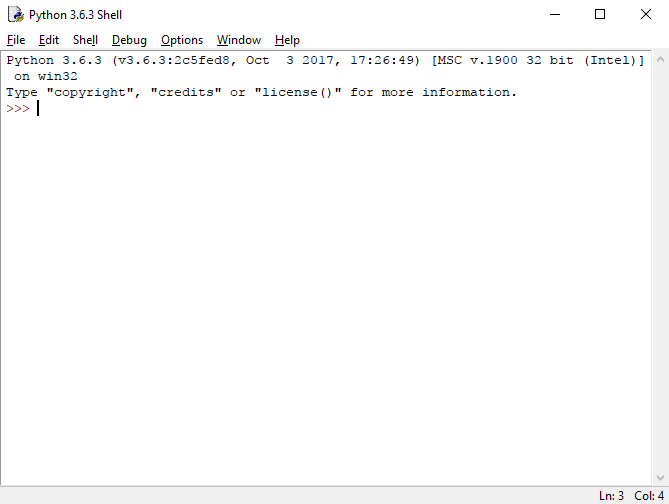
\includegraphics[width=0.8\linewidth]{McrRaspJam/016_Ciphers/1_python/idle}
		\caption{The IDLE \textit{shell} window}
		\label{fig:idle}
	\end{figure}
	
	Go to the main menu on your Raspberry Pi desktop and \textbf{open} the application titled \textit{Python 3 (IDLE)}.
	
	After a few seconds, IDLE will open to the \textit{Python Shell}. In this window, go to \textbf{File $\rightarrow$ New File}, which will open an empty window where we can write our programs.
	
	\subsection*{Hello, World!}
		
		In your empty window, \textbf{copy} the following program:
		
		\lstinputlisting[style=Python, title=helloworld.py]{McrRaspJam/016_Ciphers/1_python/helloworld.py}
		
		then, select \textbf{Run $\rightarrow$ Run Module} at the top of the window.
		
		After saving, your program will run and ``Hello, World!'' should appear in the shell window in blue.
		
	\subsection*{Inputting text}
	
		The next thing we'll need for our cipher programs is to enter text when our program runs. \textbf{Modify} your code to add the following command.
		
		\lstinputlisting[style=Python]{McrRaspJam/016_Ciphers/1_python/input.py}
		
		\textbf{Run} your program again. This time you will be asked to enter text into the shell window, and when you press enter it will be repeated back to you.
		
		\begin{aside}[Variables]
			When we store data (like text or numbers) in our programs, we store them as \textit{variables}.
			
			A variable has a \textit{label}---what the variable is called---and a \textit{value}---the data we wish to store in it.
			
			When we `set' a variable, we call this an \textit{assignment}, signified by the \texttt{=} sign.
		\end{aside}
	
	\subsection*{Lists}
	
		It is often useful to store several pieces of data in a single variable. A common way of doing this in Python is to use a list.
		
		\textbf{Open} a new file by selecting \textbf{File $\rightarrow$ New File}, then write the following program in the new window:
		
		\lstinputlisting[style=Python, title=list.py, breaklines=true]{McrRaspJam/016_Ciphers/1_python/list.py}
		
		Before you run your program, have a guess what will be printed out when you run the program. Run your program, then see whether what was printed matched what you thought it would be.
		
		\textit{extra challenge:} How can we fix the word spacing in the printed text?
		
		\begin{aside}[Lists]
			When we add \textit{elements} of data to a list, they are given the next available \textit{index} number.
			
			\vspace{4pt}
			\begin{tabular}{c|c}
				0 & Vanilla \\ 
				1 & Strawberry \\ 
				2 & Chocolate \\ 
				3 & Raspberry Ripple
			\end{tabular} 
			\vspace{4pt}
						
			To access a single element from a list, we use square brackets, as we have done in our program above.
		\end{aside}
	
	\subsection*{Strings are Lists}
	
		When we write our cipher programs, we'll need to look at single letters from the sentences we input. In python, a text \texttt{string} is actually a list of single \texttt{characters}.
		
		This means that we can access a string just like a list. Return to your hello world program, and \textbf{modify} the print statement as follows.
	
		\textbf{\lstinputlisting[style=Python, title=helloworld.py]{McrRaspJam/016_Ciphers/1_python/inputlist.py}}
		
		Now, when you run your program, only the first letter of whatever you typed in will be printed out.
		
		Next, we'll try printing out each letter one-by-one, which we can do using a \textit{loop}.
		
		\textbf{\lstinputlisting[style=Python, title=helloworld.py]{McrRaspJam/016_Ciphers/1_python/inputlist2.py}}
		
		The \texttt{for} loop we used repeats once for each element in the list that we provide it, in this case each letter in our string.
		
		\textbf{Run} your program, and this time your text should be printed one character at a time, each on its own line.
		
	
	\webclearpage
	\section{Substitution Ciphers}
	\subsection{Atbash}
	\subsection{Caesar Cipher}
	
	\section{Transposition Ciphers}
	\subsection{Scytale}
	\subsection{Railfence}
	
	\clearpage
%	\begin{appendices}
%	\end{appendices}

\end{document}